% !TeX root = ./PhDThesis.tex

\chapter{Ion trapping}
\label{chap:ion_trapping}

\section{The \texorpdfstring{${ }^{171} \mathrm{Yb}^{+}$}{} qubit}

With mass factor of 171 and nuclear spin of 1/2, ${ }^{171} \mathrm{Yb}^{+}$ has been selected as the qubit system candidate in our laboratory. Other types of ions, such as $\mathrm{Ba}^+$ \cite{RN259,RN156,RN253}, $\mathrm{Ca}^+$ \cite{RN164}, are also widely used in trapped ion experiments. In this experiment, we use the radio frequency electrical field to trap the ${ }^{171} \mathrm{Yb}^{+}$ ion. Hyperfine clock states are used to encode the qubit because they are stable against magnetic fluctuations. The two hyperfine states of the ${ }^2 \mathrm{S}_{1 / 2}$ manifold are encoded as $\left|\downarrow_z\right\rangle \equiv\left|F=0, m_F=0\right\rangle$ and $\left|\uparrow_z\right\rangle \equiv\left|F=1, m_F=0\right\rangle$. The ${ }^2 \mathrm{S}_{1 / 2} \leftrightarrow{ }^2 \mathrm{P}_{1 / 2}$ transition of the ${ }^{171} \mathrm{Yb}^{+}$ ion is nearly cyclic, but there are 0.5\% of spontaneous emission events that cause the state to decay to ${ }^2 \mathrm{D}_{3 / 2}$. Consequently, a 935 nm laser is continuously on to repump the state to ${ }^{3} [3 / 2]_{1 / 2}$ and subsequently decays back to ${ }^2 \mathrm{S}_{1 / 2}$ in order to finish the cycle transition. By addressing the transition ${ }^2 \mathrm{S}_{1 / 2} \leftrightarrow{ }^2 \mathrm{P}_{1 / 2}$ with a 370 nm laser, Doppler cooling, optical pumping and state detection may be achieved \cite{RN281}. With the use of acoustic-optic modulator (AOM) and electro-optic modulator (EOM), we put all these operations into practice.

\subsection{Two-photon ionization}

Generating an ion and loading it into the Paul trap are the first step towards a trapped-ion quantum computer. The energy necessary to ionize neutral ytterbium to ${ }^{171} \mathrm{Yb}^{+}$ ion is at least a photon with the wavelength below 198.2 nm in the FUV zone, which is hard to produce as a laser. Instead, we adopt a two-photon ionization method to produce ${ }^{171} \mathrm{Yb}^{+}$ with a single valance electron through the intermediate level ${ }^1 \mathrm{P}_1$. An enriched ytterbium atomic source can be used to produce neutral atomic flux towards the trap center. Once the flux is ejected into the trap center, a laser at 398.9110 nm illuminates the region to first ionize the atoms to a highly excited state ${ }^1 \mathrm{P}_1$ and then another laser with wavelength below 393.1 nm continuously removes the electron, leaving only a valance electron on the atomic orbits \cite{RN74,RN132,RN85}.

\begin{figure}
    \centering
    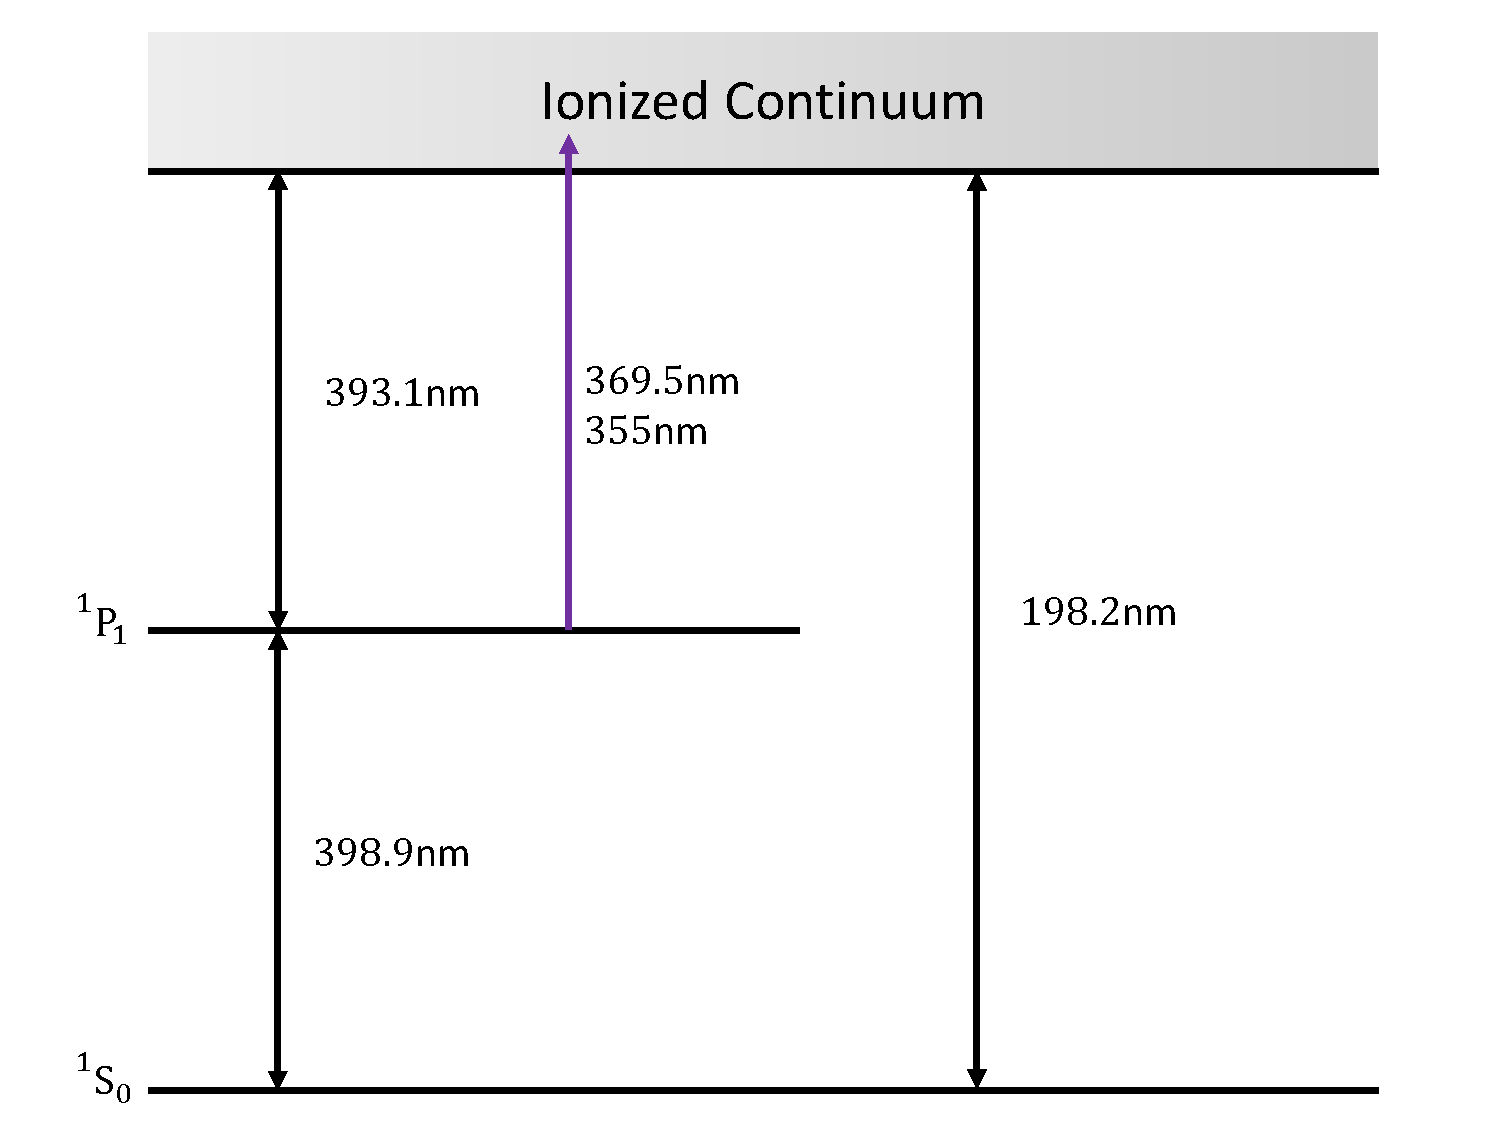
\includegraphics[width=0.5\linewidth]{fig_2_photo_ionization.pdf}
    \caption{Two-photon ionization scheme on ${ }^{171} \mathrm{Yb}^{+}$.}
    \label{fig:photo_ionization}
\end{figure}

Two-photon ionization allows for more precise control of isotope choice. The desired atomic source is often enriched, with an abundance as high as 91.7\%, the remainder consists of various natural isotopes, such as ${ }^{174} \mathrm{Yb}$, ${ }^{172} \mathrm{Yb}$, ${ }^{168} \mathrm{Yb}$ etc. We assume 50 ions in a large-scale trapped-ion quantum computer, and the average number of dark isotopes is 4. Thankfully, the intermediate level 398.91 nm transition exhibits an isotope-shift, which may be used to differentiate between isotopes. Doppler shift is a practical consideration that requires further care. The 398.91 nm laser is oriented perpendicular to the atomic flux to mitigate the Doppler effect. Isotope-selective loading of ions is possible in this setup, increasing the likelihood of the desired isotope, and this may be improved by decreasing the power of the 398.91 nm laser to achieve a narrow linewidth , although this might delay loading speed. Clock states, $\left|\downarrow_z\right\rangle \equiv\left|F=0, m_F=0\right\rangle$ and $\left|\uparrow_z\right\rangle \equiv\left|F=1, m_F=0\right\rangle$, encode the qubit. With the combination of Doppler cooling, optical pumping and state detection, we realize the cyclic transition between the $6^2 \mathrm{P}_{1 / 2}$ states and the ground state $6^2 \mathrm{S}_{1 / 2}$ \cite{RN218}. A magnetic field applied externally causes a splitting of the $|F=1\rangle$ manifolds through the Zeeman effect at a rate of roughly 1.4 MHz/G, whereas the second-order Zeeman effect dominates the clock qubits at a rate of about 310 Hz/$\mathrm{G}^2$.

Routine ion loading procedures include directing an atomic beam to the loading zone, where several laser beams are utilized to photoionize the atoms. A needle and some shards of metal are all that make up the oven, enriched in ${ }^{174} \mathrm{Yb}$ and ${ }^{171} \mathrm{Yb}$ in separate ovens. On the outside, a current loop is created by connecting the needle's head and tail with Kapton wires to the positive and negative terminals of the power supply. No part of the needle should be anchored to the floor of the chamber. That's because doing so would generate a substantial current to flow into the ground. Since current flows preferentially toward a lower potential, this phenomena may be prevented by isolating the negative poles of the current source from the ground. Keep in mind that while powering the oven for the first time, we must increase the current gradually so as not to accidentally ignite it and safeguard the SAES ion pump. The first time you use an oven, numerous grimy items will likely be fired out, which might cause the SAES ion gauge current to rise to the order of A. The atoms are expelled into the trap's central zone after the oven is heated for several minutes.

\begin{figure}
    \centering
    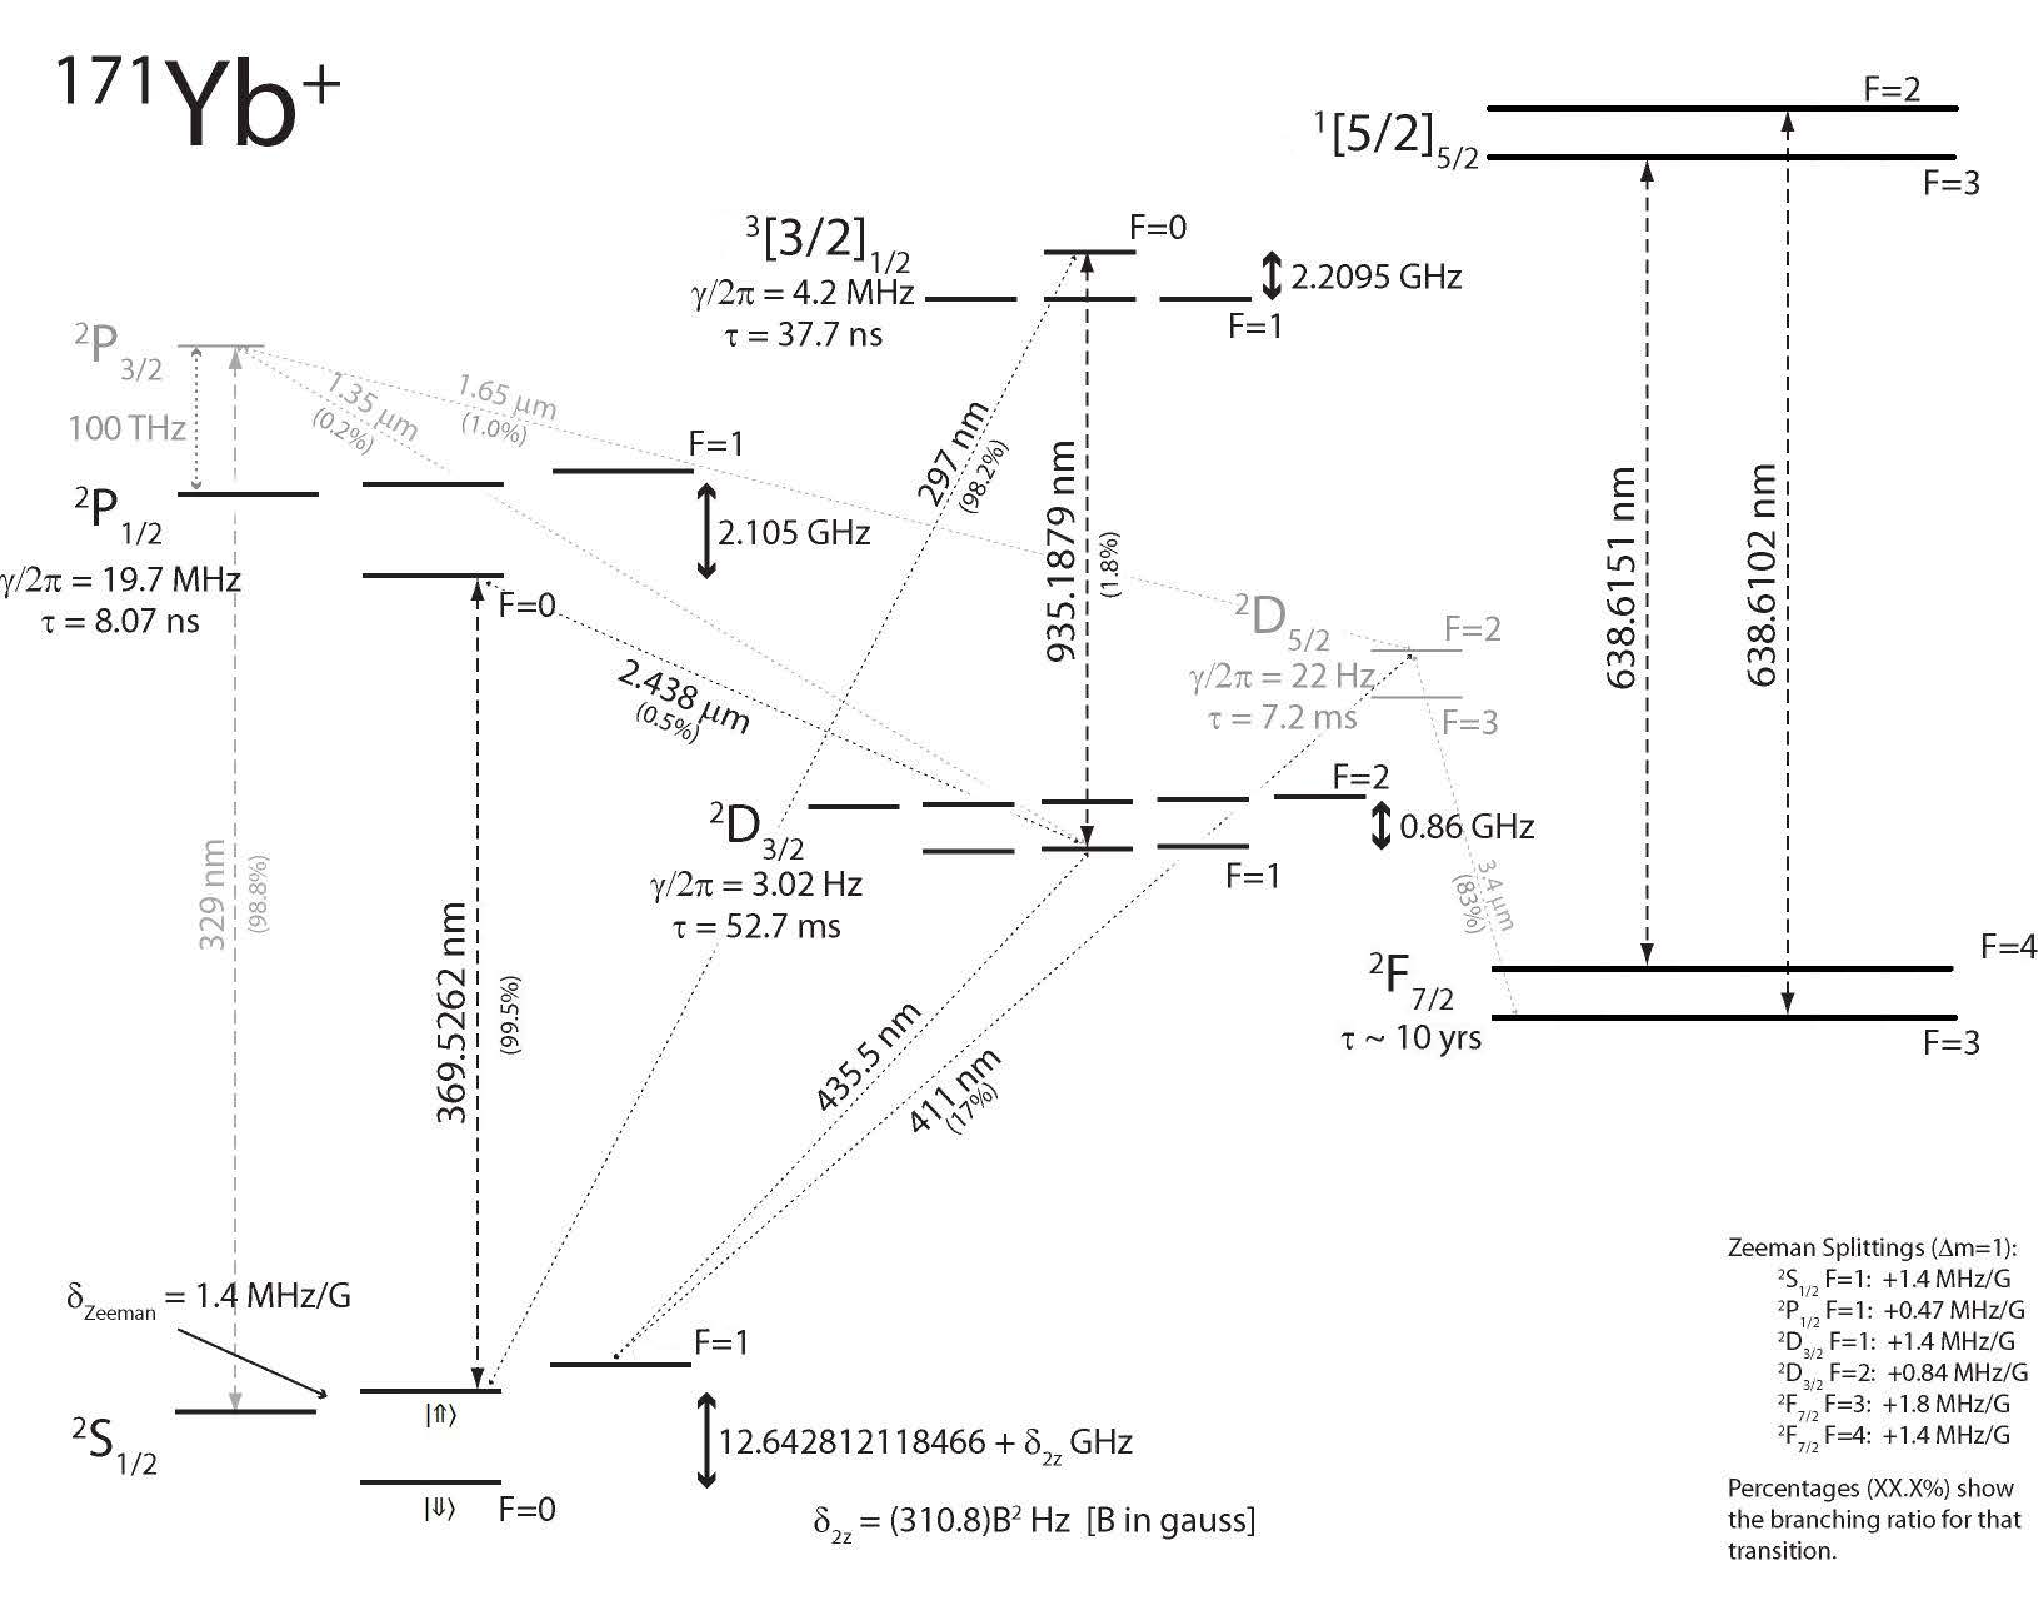
\includegraphics[width=1.0\linewidth]{fig_2_energy_level.pdf}
    \caption{${ }^{171} \mathrm{Yb}^{+}$ energy level diagram.}
    \label{fig:energy_level}
\end{figure}

\subsection{Doppler cooling}

Ions have a too wide motional area to be detected after they have been loaded into the trap since they are still very hot. We must first cool down the heated ions and produce the Coulomb crystal in order to stabilize and crystallize them. Doppler cooling \cite{RN124,RN148,RN129,RN216} is a method of rapidly cooling ions by utilizing a cyclic transition whose excited state has a very short lifetime and, therefore, a very high cooling rate. Doppler cooling is achieved in the ${ }^{171} \mathrm{Yb}^{+}$ system using a red-detuned laser to access $6^2 \mathrm{P}_{1 / 2}$ levels with a lifetime of around 8.12 ns, a natural linewidth of 19.6 MHz, and a transition of 369.5263 nm.

Doppler cooling of ions is shown in a simplified model \cite{RN152,RN154,RN243}, where ion micromotion is disregarded and the trapping potential is represented by the time-independent pseudo harmonic potential $V(z)=\frac{1}{2} m \omega_z^2 z^2$ just in the z direction. Although the trapped ion's motion is no longer in the quantum domain after Doppler cooling, it can be treated as a classical motion with a velocity that obeys $v(t)=v_0 \cos \left(\omega_z t\right)$. Let us consider the hypothetical case of a single, moving laser interacting with a trapped two-level ion consisting only of S and P states. One cycle of absorption and spontaneous emission occurs in a time period. However, the ion's velocity does not vary noticeably if the radiative decay rate of the P-level is significantly bigger than the motional frequency. In this scenario, we may represent the average radiation pressure exerted on an ion as a continuous force that varies with its speed. A photon's absorption causes an ion's momentum to increase by $\Delta \mathbf{p}=\hbar \mathbf{k}$ in the direction of the photon's wave vector, and the ion's subsequent spontaneous emission likewise increases its momentum. After many cycles of absorption and emission, the ion will be slowed when the wave vector contains a component along the direction of motion. But the direction of the momentum kick due to spontaneous emission is random across cycles.

The Doppler cooling limit $T_{\min }=\hbar \Gamma(1+\chi) /\left(4 k_B\right)$ can be achieved by laser detuning $\Delta=-\frac{\Gamma}{2}$, where $\chi$ is the geometrical factor for spontaneous emission, $\Gamma=\sqrt{1+s} \Gamma_0$ is the effective linewidth broadened by power, $s$ is the saturation parameter and the saturation intensity is $I_{\text {sat }}=\frac{\pi h c \Gamma_0}{3 \lambda^3}=510 \mathrm{~W} / \mathrm{m}^2$ \cite{RN201, RN127}. In addition, re-pumping $|\downarrow\rangle$ back to the cycled transition necessitates an additional frequency component with a detuning of 14.748 GHz. Moreover, the influence of the hyperfine levels must be taken into account, therefore a laser with a wavelength of 935.1880 nm and a sideband of 3.0695 GHz are needed. The branch ratio from level $6^2 P_{1 / 2}$ to level $5^2 D_{3 / 2}$ is non-zero at 0.5\%. Doppler cooling may be employed to achieve a final state with a phonon number below 10, where the crystal is stable against certain heating influences from the environment.

\begin{figure}
    \centering
    \subcaptionbox{Doppler cooling.}
    {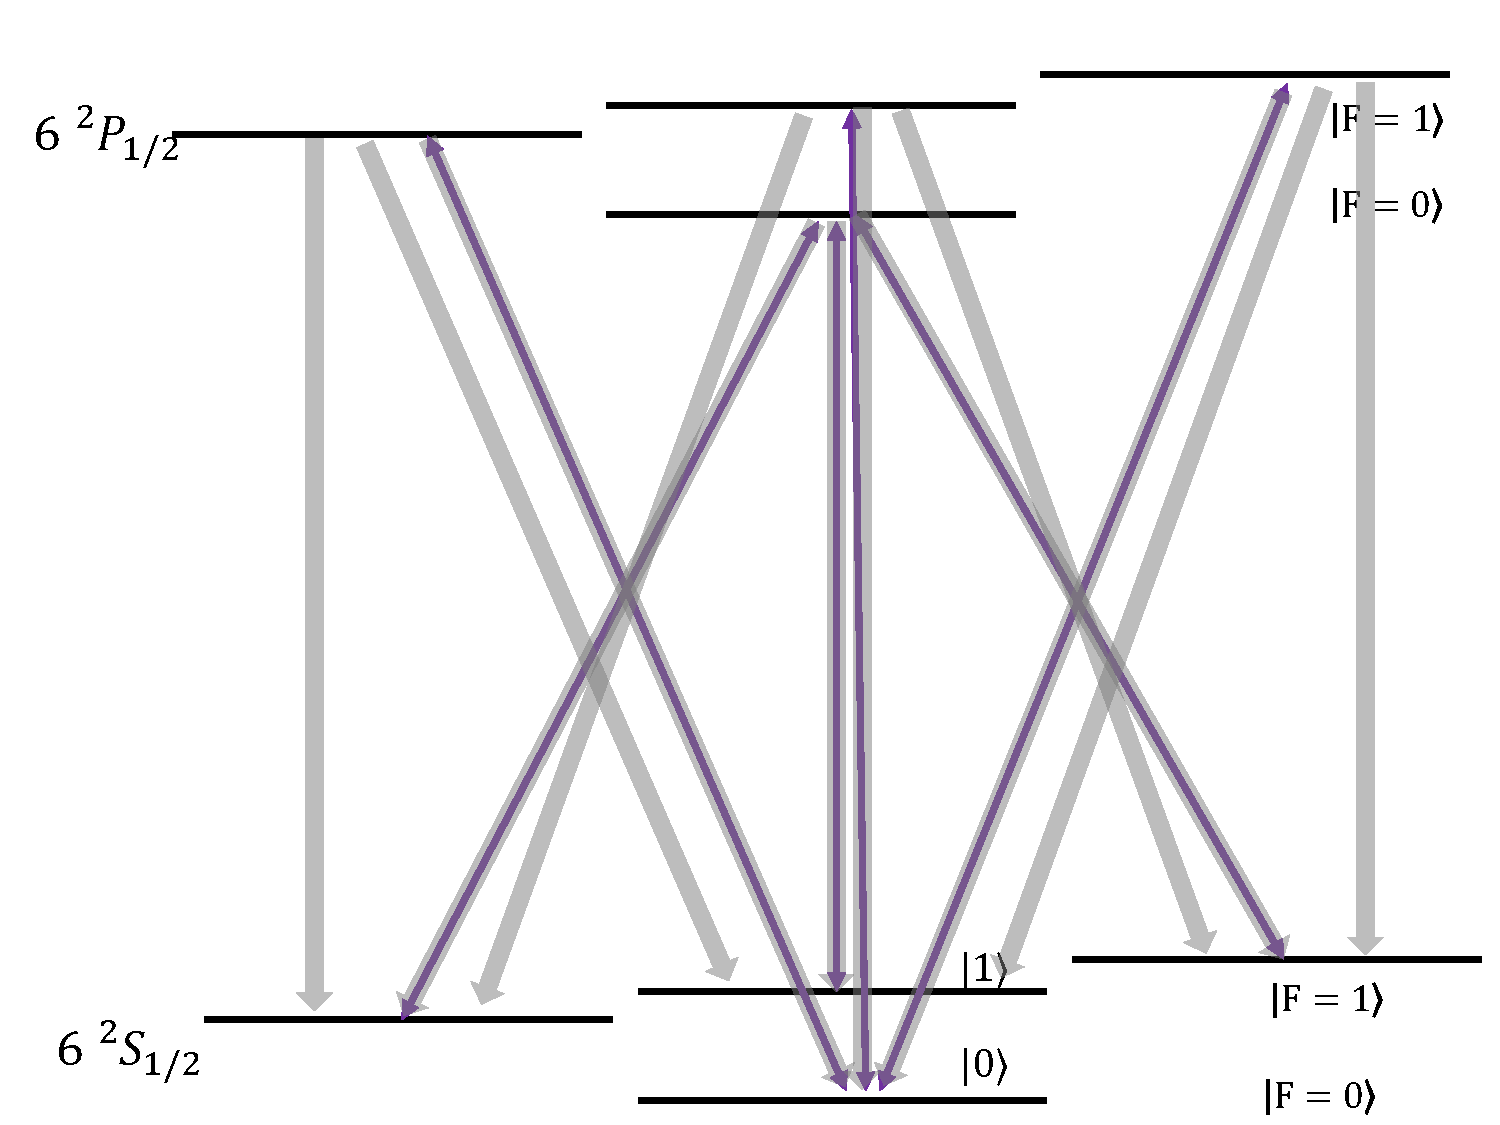
\includegraphics[width=0.4\linewidth]{fig_2_370_transitions_cooling.pdf}}
    \subcaptionbox{Optical pumping.}
    {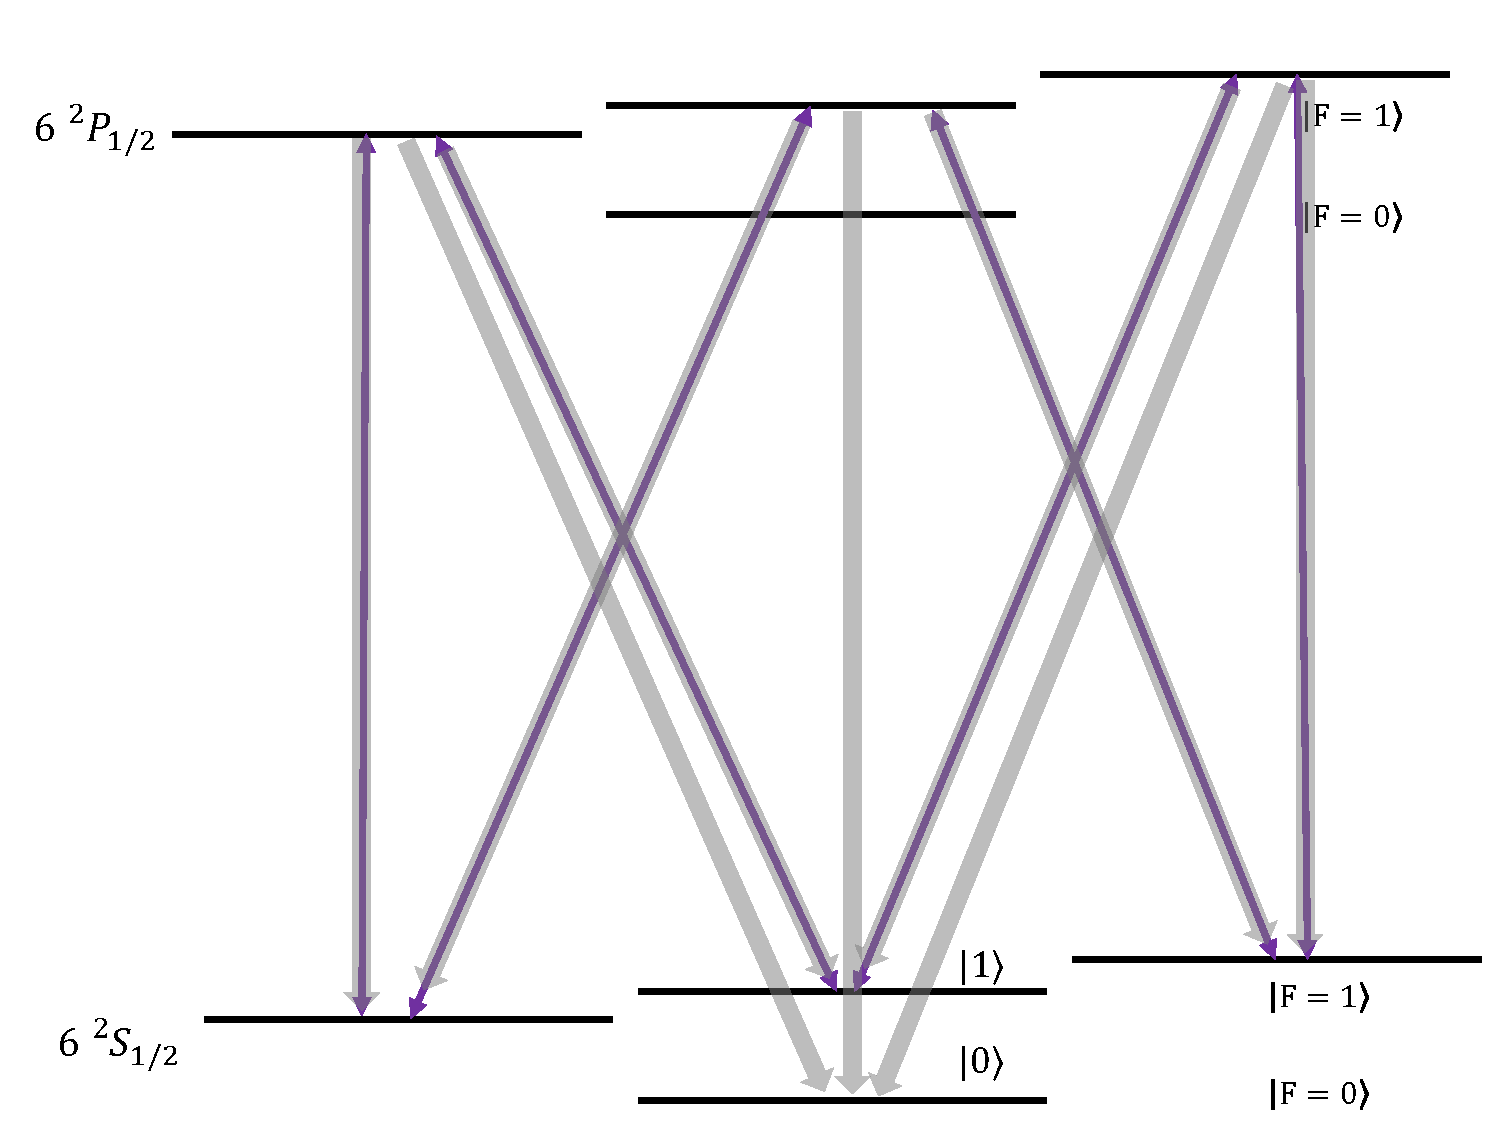
\includegraphics[width=0.4\linewidth]{fig_2_370_transitions_pumping.pdf}}
    \subcaptionbox{State detection.}
    {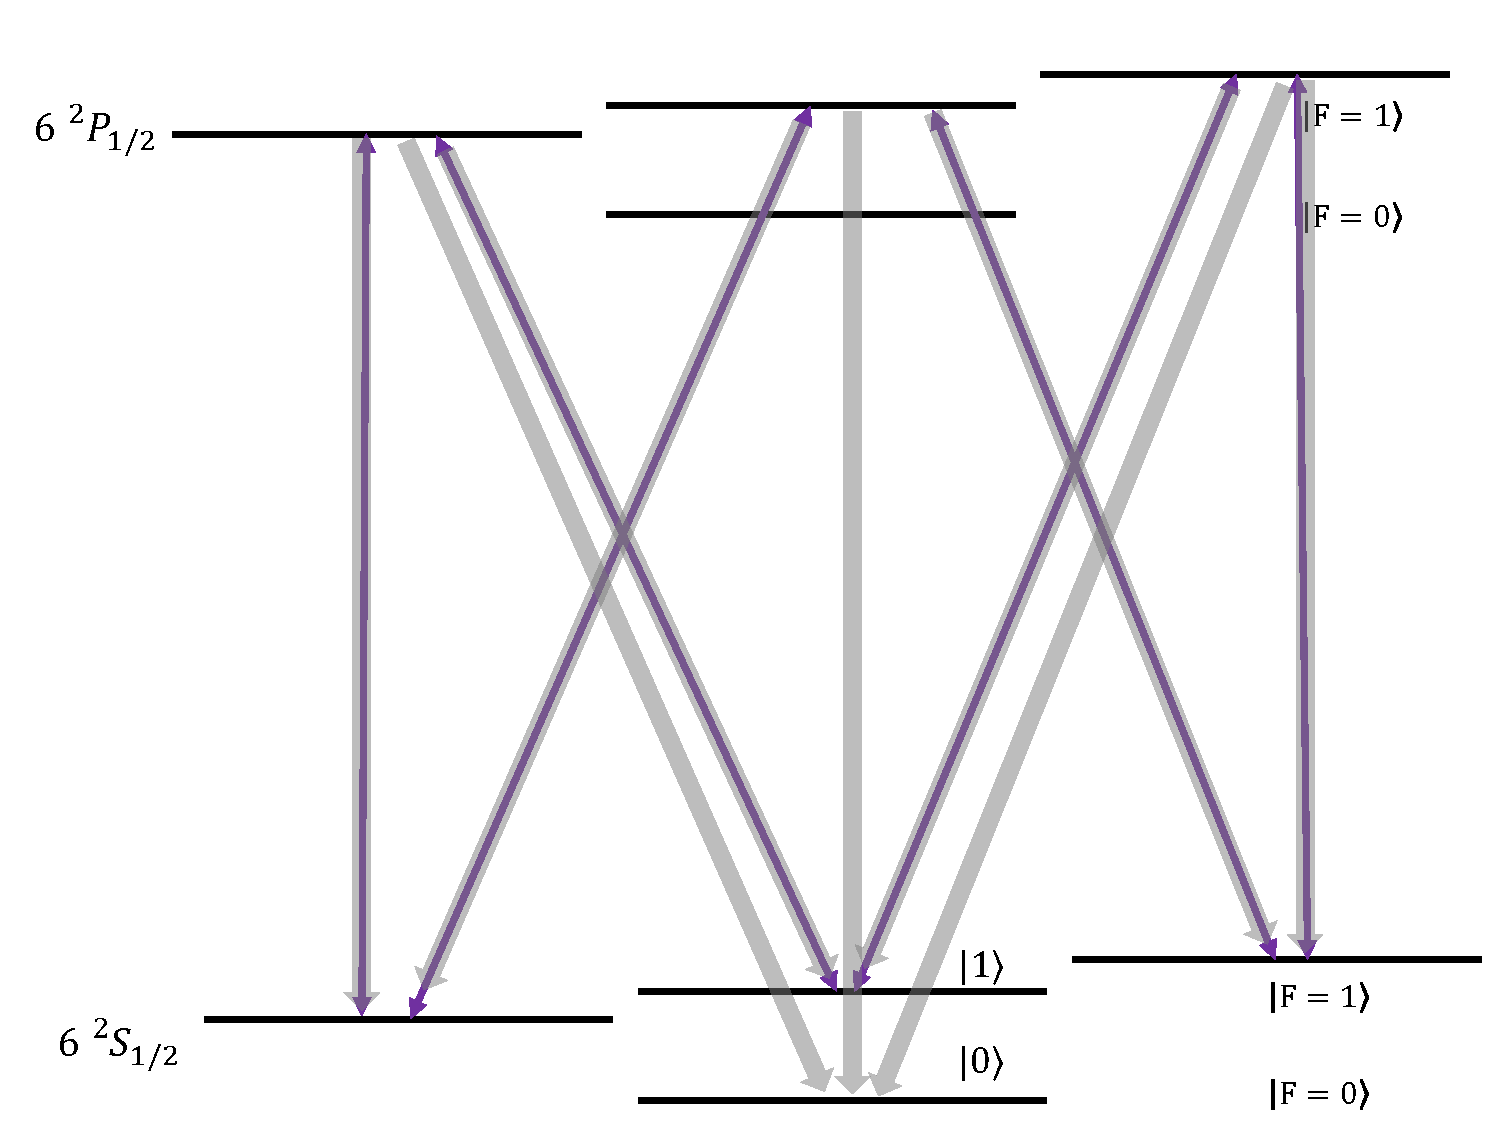
\includegraphics[width=0.4\linewidth]{fig_2_370_transitions_pumping.pdf}}
    \caption{The relevant transitions for 369.52 nm laser.}
    \label{fig:370_transitions}
\end{figure}

\subsection{Optical pumping}

When the ions have been cooled, the $\left|\downarrow_z\right\rangle$ state is prepared using optical pumping. Laser at 370 nm is stimulated when the ${ }^2 \mathrm{S}_{1 / 2} \mathrm{~F}=1$ to ${ }^2 \mathrm{P}_{1 / 2} \mathrm{~F}=1$ transition occurs. If the ion enters the ${ }^2 \mathrm{P}_{1 / 2} \mathrm{~F}=1$ manifold, it may spontaneously decay to any of the ${ }^2 \mathrm{S}_{1 / 2}$ states. The ion is around 10 GHz off resonant from the nearest transition. From the ${ }^2 \mathrm{P}_{1 / 2} \mathrm{~F}=1$ state, the ion has a 1/3 chance of decaying to the $\left|\downarrow_z\right\rangle$ state. According to the energy diagram, the optical pumping beam has to include both linear and circular components of polarization.

\subsection{State detection}

An experiment's initial step is always preparing the $\left|\downarrow_z\right\rangle$ ion chain. The next step is to actually do the experiment, followed by analysis. When the $\hat{\sigma}_z$ operator is used for measurements, the $\left|\uparrow_z\right\rangle$ and $\left|\downarrow_z\right\rangle$ states of the ions are the only viable results.

It is possible to determine the state of the ion by shining light with a wavelength of 370 nm onto an ion chain that is resonant with the ${ }^2 \mathrm{S}_{1 / 2} \mathrm{~F}=1$ to ${ }^2 \mathrm{P}_{1 / 2} \mathrm{~F}=0$ transition. This kind of light is known as a detecting light. The detecting light will only resonate with the $\left|\uparrow_z\right\rangle$ state if it is present. It is possible for the ion to decay spontaneously to any of the ${ }^2 \mathrm{S}_{1 / 2} \mathrm{~F}=1$ levels. Since it is desirable to have numerous absorption or emission events, the beam has all possible polarization components. This allows the detection process to continue without interruption until sufficient photons have been gathered to determine the ion state \cite{RN221,RN298,RN104,RN222}. The ion fluoresces isotropically when exposed to the detecting light. And a portion of the light that is emitted by the ion is gathered by imaging optics and directed onto an EMCCD camera in order to read out the spin state. The detection light has a minuscule chance of off-resonantly exciting either spin state to the ${ }^2 \mathrm{P}_{1 / 2} \mathrm{~F}=1$ manifold, where the ion may subsequently decay into the other spin state and induce detection errors \cite{RN235}. This happens because of the ${ }^2 \mathrm{P}_{1 / 2} \mathrm{~F}=1$ manifold.

Doppler cooling, optical pumping, and state detection are all examples of operations that entail spontaneous decay to the ${ }^2 \mathrm{S}_{1 / 2} \mathrm{~F}=1$ manifold of states \cite{RN215}. Hence, if the Zeeman states are degenerate, the mechanism of coherent population trapping may be used to pump the ion into a dark state. As a result, an application of a B-field is made to the ions in order to disrupt this degeneracy and stop the trapping of coherent populations. In the location where the ions are located, the B-field strength is 5 G, and the Zeeman splitting from the $\left|\uparrow_z\right\rangle$ state is measured 12 MHz.

We are able to determine the state of the spins in the ion chain by capturing the spin-dependent fluorescence using a site-resolving image Andor iXon Ultra 888 EMCCD camera. During the state detection process, a resonant laser with a wavelength of 370 nm is shone between $\left|\uparrow_z\right\rangle$ and $\left|\downarrow_z\right\rangle$. When the qubit is in the $\left|\downarrow_z\right\rangle$ state, a small amount of photons are scattered off. However, when the spin state is in the $\left|\uparrow_z\right\rangle$ state, a significant number of photons are scattered off. The binary threshold for spin-state discrimination is determined by calibrating the number of photons dispersed from the bright $\left|\uparrow_z\right\rangle$ state and the dark $\left|\downarrow_z\right\rangle$ state of each spin at the beginning of the process of collecting data on those spins. The bright and dark states of the setup used in this thesis have an average fidelity of more than 97 \%, which is suitable for the quantum memory experiments. The off-resonant mixing of spin states during detection, crosstalk between nearby ions, noise from the electronic camera, and noise from the laser are the primary causes of mistake in this case \cite{RN128}.


\section{The linear Paul trap}

According to one of Maxwell's equations, $\nabla \cdot \vec{E}=0$, the electric field will not diverge in a region where there is no free charge density. This conclusion may be drawn from the fact that: Earnshaw deduced from this equation that it was mathematically impossible for a charged particle to be connected in a static electric field in all directions at the same time. Yet, in order to condense charged particles, either oscillating electric fields or a combination of static electric and magnetic fields are required. In this experiment, the RF trap is the primary focus.

Assuming for the sake of this discussion that the ions have a positive charge, mathematically express the criteria of an accessible potential that requires minima in any direction as shown below.
\begin{equation}\label{eq:minima}
    \frac{\partial \mathbf{E}}{\partial x_i}=-\frac{\partial^2 \Psi}{\partial x_i^2}<0, x_i \in\{x, y, z\}.
\end{equation}

However, Eq.~\eqref{eq:minima} contradicts of the Laplacian equation for static electric fields in vacuum, which states that else there would never be a global minimum in any of the directions otherwise $\frac{\partial \mathbf{E}}{\partial x_i}=0$.
\begin{equation}
    \nabla^2 \Psi=0.
\end{equation}

The ion trap technique, which uses a mix of DC and RF oscillating electric fields, offers a fortunate alternative to the traditional method of confining ions in a vacuum environment. It is possible to write down the broad potential of a Paul trap as
\begin{equation}\label{eq:rfpotential}
    \Psi(x, y, z)=\frac{U}{2}\left(\alpha x^2+\beta y^2+\gamma z^2\right)+\frac{V}{2} \cos (\Omega t)\left(\alpha^{\prime} x^2+\beta^{\prime} y^2+\gamma^{\prime} z^2\right),
\end{equation}

$\alpha, \beta, \gamma, \alpha^{\prime}, \beta^{\prime}, \gamma^{\prime}$ are geometrical factors. This kind of potential may be generated using hyperbolic electrodes, the geometrical factors involved are precisely $1 / r^2$, where $r$ denotes the distance to the electrodes. Unfortunately, the hyperbolic electrodes restrict the optical access. There are some novel designs for traps with high optical access, but the geometrical considerations need to take into account the approximations that are necessary since the hyperbolic electrodes are not ideal. There is an extra restriction for the geometrical factors that must be satisfied in order to satisfy the Laplacian equation
\begin{equation}
    \alpha+\beta+\gamma=0,\quad \alpha'+\beta'+\gamma'=0.
\end{equation}

To be more specific, a Paul trap with the parameters $\gamma^{\prime}=0, \alpha=\beta=-\frac{\gamma}{2}, \alpha^{\prime}=-\beta^{\prime}$ is referred to as a linear trap. In a linear trap, charged particles are only confined by a static field in one direction, while RF fields are used to confine them in the other two directions.

\subsection{Mathieu equation}

With a Paul trap, it is possible to decouple the motion of charged particles in three different directions. In this case, we will treat in $x$ for the sake of simplicity following,
\begin{equation}\label{eq:motion}
    m \frac{\mathrm{d}^2 x}{\mathrm{~d} t^2}=-Q\left(\alpha U x+\alpha^{\prime} V \cos (\Omega t) x\right),
\end{equation}

substitute $\tau=\frac{\Omega t}{2}, a_x=\frac{4 Q U \alpha}{m \Omega^2}, q_x=\frac{2 Q V \alpha^{\prime}}{m \Omega^2}$. Eq.~\eqref{eq:motion} can be simplified as a Mathieu equation
\begin{equation}
    \frac{\mathrm{d}^2 x}{\mathrm{~d} \tau^2}+\left(a_x x-2 q_x \cos (2 \tau) x\right)=0.
\end{equation}

In this case, the solution of the lowest order is shown together with the assumptions that $\left|a_x\right|, q_x^2 \ll 1$,
\begin{equation}
    \beta_x=\sqrt{a_x+\frac{q_x^2}{2}}, \quad x(t)=2 A C_0 \cos \left(\beta_x \frac{\Omega t}{2}\right)\left[1-\frac{q_x}{2} \cos (\Omega t)\right].
\end{equation}

This is a bounded solution with periodic frequency $\omega_x=\frac{\beta_x \Omega}{2}$, which is often referred to as secular motion. The second component in frequency $\Omega \pm \omega_x$ represents the intrinsic micromotion that is induced by the RF fields.

In a further approximation, it is possible to construct an effective time-independent potential to describe the dynamics of charged particles in an RF Paul trap. An example in $x$ is presented below, and we assume that the charge is equal to $e$.
\begin{equation}
    E(x, t)=E_0(x) \cos (\Omega t),
\end{equation}
\begin{equation}
    F(x, t)=m \ddot{x}=e E_0(x) \cos (\Omega t),
\end{equation}
where $E_0(x)$ is independent of the time-varying potential and solely depends on positional information. Imagine a crystal that has been stabilized such that all of its ions remain in close proximity to their positions of equilibrium. The only new vibrations that occur are those that are caused by the RF fields.
\begin{equation}\label{eq:staticmotion}
    x=x_0-\frac{eE_0(x_0)}{m\Omega^2}\cos(\Omega t).
\end{equation}

This is the first-order solution to the motion, and we may do additional Taylor expansion at the equilibrium location $x_0$ to the electric field as well, although this is not necessary.
\begin{equation}
    \begin{aligned}
        E_0(x) & =E_0\left(x_0\right)+\left.\frac{\partial E_0(x)}{\partial x}\right|_{x_0}\left(x-x_0\right)                                                    \\
               & =E_0\left(x_0\right)-\left.\frac{\partial E_0(x)}{\partial x}\right|_{x_0}\left(\frac{e E_0\left(x_0\right)}{m \Omega^2} \cos (\Omega t)\right) \\
               & =E_0\left(x_0\right)-\left.\frac{e}{2 m \Omega^2} \frac{\partial E_0^2(x)}{\partial x}\right|_{x_0} \cos (\Omega t)
    \end{aligned}
    .
\end{equation}
\begin{equation}
    \begin{aligned}
        F(x, t)=m \ddot{x} & =e E_0\left(x_0\right) \cos (\Omega t)-\left.\frac{e^2}{2 m \Omega^2} \frac{\partial E_0^2(x)}{\partial x}\right|_{x_0} \cos ^2(\Omega t)        \\
                           & =e E_0\left(x_0\right) \cos (\Omega t)-\left.\frac{e^2}{2 m \Omega^2} \frac{\partial E_0^2(x)}{\partial x}\right|_{x_0}(1+\cos (2 \Omega t)) / 2
    \end{aligned}
    .
\end{equation}

Assess the influence on average, excluding out the variables that are rapidly fluctuating,
\begin{equation}
    \bar{F}(x)=-\left.\frac{e^2}{4 m \Omega^2} \frac{\partial E_0^2(x)}{\partial x}\right|_{x_0},
\end{equation}
where \(E_0(x)=-\alpha'V x\) for the general potential. It is a harmonic confinement that does not rely on whether the ions are positively or negatively charged, and it controls the secular motion of ions inside the trap. Additional words include the source of micromotion, which has an oscillation that is much more rapid and is defined by frequency \(\Omega\). Hence, one way to define the pseudo potential is as follows,
\begin{equation}\label{eq:pseudo_potential}
    \Psi_{ps}=\frac{e}{4m\Omega^2}E_0^2(x)=\frac{e\alpha'^2V^2}{4m\Omega^2}x^2,
\end{equation}

This re-creates the conclusion that Earnshaw's theorem came to. It is a valid approximation for equilibrium positions and secular motion of charged particles in an RF trap, and it can be used to calculate the principal axes taking both DC and RF fields into account. The secular frequency is \(\omega_x=\frac{e\alpha' V}{\sqrt{2}m\Omega}\), which is consistent with the Mathieu equation. The static confinement can also be taken into account, which is also a harmonic term.

\subsection{Normal modes}

Since the normal modes are entirely decoupled from all directions, particularly the transverse modes that we are working on, we employ a chain of trapped ${ }^{171} \mathrm{Yb}^{+}$ ions as the quantum memory in a linear Paul trap \cite{RN57,RN27,RN55,RN60,RN110,RN56}. This allows us to study the transverse modes. It is necessary for the trap frequencies to adhere to the relation Eq.~\eqref{eq:linear_chain} if the Coulomb crystal is to be contained inside a linear chain.
\begin{equation}\label{eq:linear_chain}
    \left(\frac{\omega_r}{\omega_z}\right)^2 \geq \frac{N^{1.73}}{2.53},
\end{equation}
where \(N\) is the number of ions, \(\omega_r\) refers to either the transverse mode \(\omega_x\) or \(\omega_y\), and \(\omega_z\) refers to the axial mode with DC confinement.

Instead of using the straightforward Mathieu equation, one needs take into consideration the Coulomb interaction that occurs between the ions when there are a greater number of ions fed into the trap. Both the externally imposed pseudo potential and the Coulomb interactions that occur between the ions work together to decide the shape of the ion crystal.

The inter-ion spacings would not be uniform under a harmonic potential similar to Eq.~\eqref{eq:rfpotential}, where spacings at the center of an ion chain would be much more tight but loose at the edge. This would require much higher RF potential or lower DC potential to satisfy Eq.~\eqref{eq:linear_chain}, or else there would be an unstable transition to zig-zag mode. Here, we consider \(N\) ions in order to solve the issue, quartic potential is required. This is because increasing the number of electrodes along the z-axis will bring the inter-ion spacings closer to being uniform. As the micromotion is negligible in comparison to the secular motion and all of the ions are aligned with the RF null in the required configuration, the property of the ion crystal may be obtained using the pseudo potential while ignoring the time-dependent RF potential.

The potential in its broadest sense may be expressed as
\begin{equation}
    U=\sum_i\left(\frac{\alpha}{2} z_i^2+\frac{\beta}{4} z_i^4\right)+\sum_{i<j} \frac{e^2}{4 \pi \epsilon_0\left|z_i-z_j\right|}.
\end{equation}

Here, we will define the length unit known as $l=\left(e^2 / 4 \pi \epsilon_0 \alpha\right)^{1 / 3}$, and after that, we will be able to rewrite the potential \(u_i\equiv z_i/l\) using dimensionless coordinates and dimensionless energy \(U'\equiv 4\pi \epsilon_0 lU/e^2\), respectively.
\begin{equation}
    U^{\prime}=\sum_i\left(\frac{1}{2} u_i^2+\frac{\beta l^2}{4 \alpha} u_i^4\right)+\sum_{i \neq j} \frac{\operatorname{sgn}(\alpha)}{2\left|u_i-u_j\right|}.
\end{equation}

When we have ascertained the total number of ions and the potential configuration \(\frac{\beta l^2}{\alpha}\), we will be able to locate the equilibrium locations by minimizing the energy required to do so. Instead, we might try to solve the gradient equations when the system is at equilibrium.
\begin{equation}
    0=\frac{\partial U^{\prime}}{\partial u_i}=u_i+\frac{\beta l^2}{\alpha} u_i^3-\operatorname{sgn}(\alpha) \sum_{i \neq j} \frac{u_i-u_j}{\left|u_i-u_j\right|^3}.
\end{equation}

We can further reduce the problem to find the solutions of the gradient equations, which is something that can be easily accomplished by some built-in functions of Wolfram Mathematica such as FindRoot or NSolve. As an alternative to performing the optimization with multiple variables, we can use this method.

When the equilibrium locations have been determined, the Hessian matrix may be used to calculate the axial motional modes
\begin{equation}
    \frac{\partial^2 U^{\prime}}{\partial u_i \partial u_j}= \begin{cases}1+\frac{3 \beta l^2}{\alpha} u_i^2+\sum_{k \neq i} \frac{2 \operatorname{sgn}(\alpha)}{\left|u_i-u_k\right|^3}, & i=j \\ -\frac{2 \operatorname{sgn}(\alpha)}{\left|u_i-u_j\right|^3}, & i \neq j\end{cases}.
\end{equation}

Things would turn out differently with regard to the transverse modes. The COM mode has the maximum frequency, and its bandwidth is quite close to that of the axial COM mode; hence, the transverse modes have a significantly higher population density. Moreover, we are able to include the transverse words into the general form.
\begin{equation}
    U=\sum_i\left(\frac{\alpha}{2} z_i^2+\frac{\beta}{4} z_i^4+\frac{1}{2} m \omega_x^2 x_i^2+\frac{1}{2} m \omega_y^2 y_i^2\right)+\sum_{i<j} \frac{e^2}{4 \pi \epsilon_0\left|\mathbf{r}_{\mathbf{i}}-\mathbf{r}_{\mathbf{j}}\right|}.
\end{equation}

For a linear chain configuration, the equilibrium positions for transverse \(x,\, y\) are quite clear that \(x_0=0,\,y_0=0\), and we can use the same dimensionless unit \(l\) to simplify the potential expression using notation \(uz=z/l,\, ux=x/l,\, uy=y/l\).

The equilibrium positions for transverse \(x\) and \(y\) in a linear chain configuration are quite obvious: \(x_0=0,\,y_0=0\). We can use the same dimensionless unit, \(l\), to simplify the potential expression by notating it as follows: \(uz=z/l,\, ux=x/l,\, uy=y/l\). For a linear chain configuration, the equilibrium positions for transverse \(x\) and \(y\) are quite obvious.
\begin{equation}
    \begin{aligned}
        U^{\prime} & =\sum_i\left(\frac{1}{2} u z_i^2+\frac{\beta l^2}{4 \alpha} u z_i^4+\frac{m \omega_x^2}{2 \alpha} u x_i^2+\frac{m \omega_y^2}{2 \alpha} u y_i^2\right)+\sum_{i \neq j} \frac{\operatorname{sgn}(\alpha)}{2\left|\mathbf{u}_{\mathbf{i}}-\mathbf{u}_{\mathrm{j}}\right|} \\
                   & =U_0+\sum_i\left(\frac{m \omega_x^2}{2 \alpha} u x_i^2+\frac{m \omega_y^2}{2 \alpha} u y_i^2\right)-\operatorname{sgn}(\alpha) \sum_{i \neq j} \frac{\left(u x_i-u x_j\right)^2+\left(u y_i-u y_j\right)^2}{4\left|u z_i-u z_j\right|^3}
    \end{aligned}
    ,
\end{equation}
where \(U_0\) is the one only related to coordinates \(uz_i\)'s. When thinking about the transverse modes, we don't need to take them into account at all since we may ignore them. We may also derive the Hessian matrix for \(x,\, y\), and the results for \(x\) are shown below. As the right hand side of the potential has the same dependency on the sign of \(\alpha\), we can, in practice, use the absolute value instead.
\begin{equation}
    \frac{\partial^2 U^{\prime}}{\partial u x_i \partial u x_j}= \begin{cases}\frac{m \omega_x^2}{|\alpha|}-\sum_{k \neq i} \frac{1}{\left|u z_i-u z_k\right|^3}, & i=j \\ \frac{1}{\left|u z_i-u z_j\right|^3}, & i \neq j\end{cases}.
\end{equation}

\subsection{Micromotion minimization}

Ions in Paul's tarp will go through a process known as forced motion, which is driven by the frequency referred to as \(\Omega\). Some of this motion is an intrinsic effect caused by the RF potential, while other motion is caused by forced motion for ions going through a process known as nonzero oscillating force. The force may be created by a residual DC field that moves the ions away from the RF null, and the real-time electric field is not zero. The temporal dependency of the real-time electric field's frequency is characterized by \(\Omega\). The motion of ions may, as a matter of course, be explained by the linear superposition of two portions.
\begin{equation}\label{eq:excess_micromotion}
    \begin{aligned}
        \ddot{x} & =-\omega_x^2 x-\frac{E_0\left(x_0\right) e}{m} \cos (\Omega t),                    \\
        x(t)     & =A \cos \left(\omega_x t\right)+B\left(E_0\left(x_0\right)\right) \cos (\Omega t).
    \end{aligned}
\end{equation}

The periodic force will cause the second term of the solution of \(x(t)\), which is given by pseudo potential approximation. The term \(B(E_0(x_0))\) is the amplitude of excess micromotion, and it dependends on the strength of the residual electric field \(E_0(x_0)\) or the equilibrium position from RF null \(x_0\). In addition, the intrinsic micromotion that is solved by the Mathieu equation is characterized by the frequency \(\Omega\pm \omega_x\), and it is related to the transverse secular motion. On the other hand, the excess micromotion are detached from the secular motion. In addition, excess micromotion is degenerate in three directions, and in order to link the micromotion, we require a number of lasers that are not parallel to one another.

In addition to the equation that is described in Eq.~\eqref{eq:excess_micromotion}, we are able to utilize the Mathieu equation to determine the motion of the ions in the presence of a stray field, and this motion may be written as
\begin{equation}
    \begin{aligned}
        x(t) & =\left(\frac{e E_R}{m \omega_x^2}+A \cos \left(\omega_x t\right)\right)\left(1+\frac{q_x}{2} \cos (\Omega t)\right)                                                      \\
             & =A \cos \left(\omega_x t\right)+\frac{e E_R q_x}{2 m \omega_x^2} \cos (\Omega t)+\frac{A q_x}{2} \cos \left(\omega_x t\right) \cos (\Omega t)+\frac{e E_R}{m \omega_x^2}
    \end{aligned}
    .
\end{equation}

As can be seen in the figure referenced above, there are four different terms: secular motion, excess micromotion, intrinsic micromotion, and equilibrium position displacement, respectively. Because intrinsic micromotion is born with the RF potential, its amplitude can never be reduced by tinkering with the DC configurations. This is because intrinsic micromotion is only related to the RF potential and the Doppler cooling limit. For secular motion, the amplitude is related to the process of cooling, and \(\omega_x=\sqrt{a_x+\frac{q_x^2}{2}}\frac{\Omega}{2}\) for the intrinsic micromotion. It is obvious that the excess micromoiton is associated with the stray field that is exerted on the ions. This amplitude is proportional to \(a_x<<q_x^2\), in particular for transverse modes in an ion chain. And it can be easily demonstrated that the amplitude will be reduced when increasing the RF level. In addition to this, the ion position will approach the RF null space by factor \(\frac{1}{a_x+\frac{q_x^2}{2}}\).

Expanding the electric field is possible within the context of the rotating frame of the ions' secular motion,
\begin{equation}
    E(x, t)=E_0 e^{-i\left(\omega_0 t-k_x x(t)\right)}=E_0 e^{i k_x A \cos \left(\omega_x t\right)\left(1+\frac{q_x}{2} \cos (\Omega t)\right)} e^{-i\left(\omega_0 t-\frac{k_x e E_R q_x}{2 m \omega_x^2} \cos (\Omega t)\right)}.
\end{equation}

So, we are able to make use of the modulation information in order to extract the amplitude of excess micromotion, and the RF modulation may also regulate the fluorescence. A cooling laser is used in this technique to detect the modulation, and of course, non-parallel lasers are required in order to reconstruct the full information of excess micromotion. The fluorescence can be demodulated by using a device called a time-arrival-converter, but this method has some drawbacks. Unfortunately, because of the geometry of the chamber, it is not always possible to send lasers in all three directions, and this difficulty might be considerably more severe for surface planar traps, particularly when the cooling laser is operating in the ultraviolet range. A combination of Raman sideband and EMCCD monitoring ion position is another method that may be used to identify excess micromotion.

In this article, we present the parametric excitation approach for the purpose of minimizing excess micromotion because of its ease of use and high degree of accuracy \cite{RN101,RN130,RN200,RN122,RN112}. Although the delivery of laser along the objective might be challenging, the accuracy of micromotion minimization along the objective is completely constrained by the resolution and amplification capabilities of the imaging system. This was covered in the previous section. To be able to detect extra micromotion in any of the three orthogonal directions, parametric excitation just needs a single cooling beam to readily connect to all three directions simultaneously \cite{RN79,RN123,RN111,RN113}. It is possible to put it into practice by modulating the amplitude of RF fields, using the pseudo potential approximation, the force that is exerted on the ions is
\begin{equation}\label{eq:parametric_excitation}
    \frac{\mathrm{d}^2 \bar{x}}{\mathrm{~d} t^2}+\xi \frac{\mathrm{d} \bar{x}}{\mathrm{~d} t} \omega_x^2\left(1+2 h \cos \left(\omega_m t\right)\right) \bar{x}=\frac{e E_R}{m},
\end{equation}
where \(h\) is the modulation index,
\begin{equation}
    E(r,t)=E_0(r,t)(1+h\cos(\omega_m t)),
\end{equation}
the corresponding pseudo potential is proportional to
\begin{equation}
    E^2(r,t)=E_0^2(r,t)(1+2h\cos(\omega_m t)),
\end{equation}
and \(\xi\) is the damping coefficient of the cooling beam.

The parametric excitation, in contrast to the forced oscillation, will not take place if the initial condition \(\bar{x}(0)=0\), and the parametric excitation will only be excited at the modulation frequency \(\omega_m=\frac{2\omega_x}{n}\), where \(n\) is a positive integer. The forced oscillation will take place regardless of the initial condition. Depending on the experimental regime, the parametric excitation will either induce a decrease in fluorescence or an increase in it. So, the parametric excitation may be utilized to identify excess micromotion if ions are pushed away from the RF null. Nevertheless, once \(\bar{x}\) approaches the equilibrium location of the RF null, the parametric excitation will cease to exist.

In addition, a recent piece of research demonstrates that there is a link between the fluorescence and the amplitude modulation signal. In this example, we will show how parametric excitation may occur when \(\omega_m=\omega_x\). The stable solution may be derived by using Floquet theory even in the absence of explicit derivations, which take into account corrections for secular frequency and modulation depth.
\begin{equation}
    \bar{x}(t)=\sum_nc_ne^{ic_n\omega_mt},
\end{equation}
\(c_n=c_{-n}^*\) for symmetry, and \(c_0\) depends on the first order of modulation, \(c_0=\frac{eE_R}{m\omega_x^2}\).

Then we can extend it to the second order. We can simplify
\begin{equation}
    \bar{x}(t)=c_0+2 \Re\left(c_{-1} e^{-i \omega_m t}\right).
\end{equation}
If we replace it back into Eq.~\ref{eq:parametric_excitation}, we can easily find the answer for the second order,
\begin{equation}
    |c_{-1}|^2=\frac{2 c_0^2 h^2}{\left(f^2-1\right)+4 f^2 d^2}, \quad \tan \left(\arg \left(c_{-1}\right)\right)=\frac{2 f d}{f^2-1},
\end{equation}
where \(f=\frac{\omega_m}{\omega_x},\, d=\frac{\xi}{\omega_x}\) are normalized frequency and damping factor. The amplitude of \(c_{-1}\) is linearly proportional to \(c_0\), and thus \(E_R\).

\begin{figure}
    \centering
    \subcaptionbox{Correlated signal in the x-axis ($\omega_x$).}
    {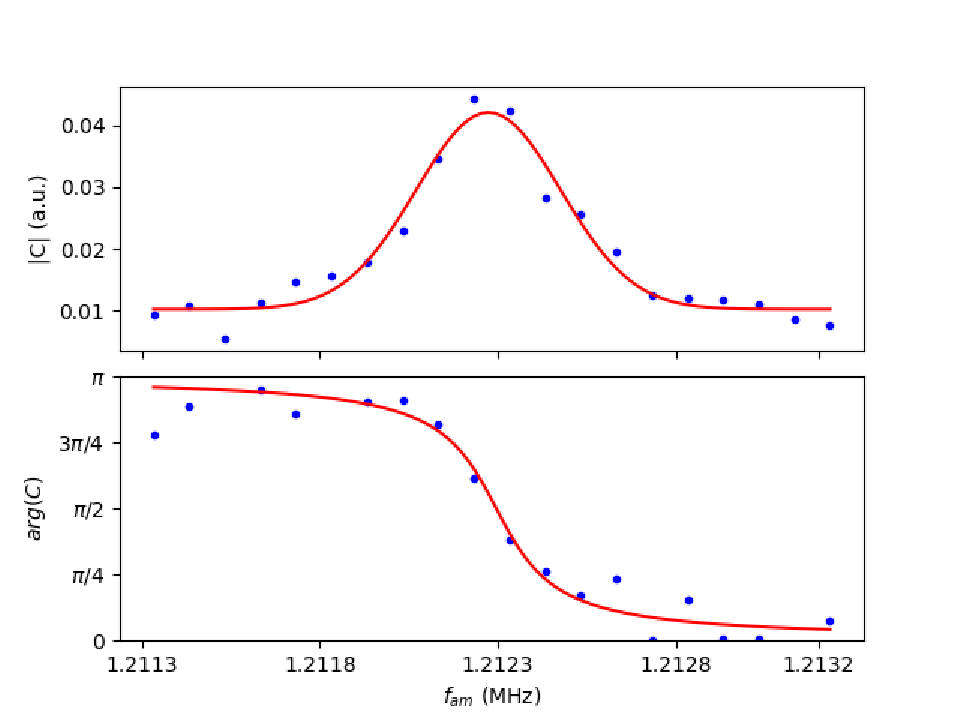
\includegraphics[width=0.4\linewidth]{fig_2_pe_x.pdf}}
    \subcaptionbox{Correlated signal in the y-axis ($\omega_y$).}
    {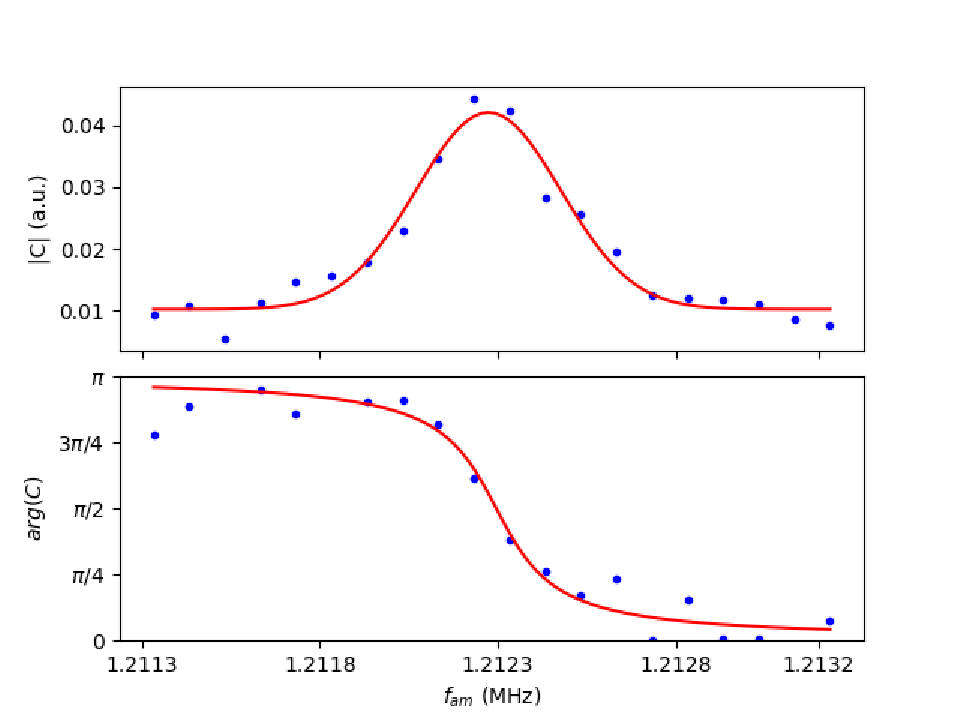
\includegraphics[width=0.4\linewidth]{fig_2_pe_x.pdf}}
    \subcaptionbox{Correlated signal in the z-axis ($\omega_z$).}
    {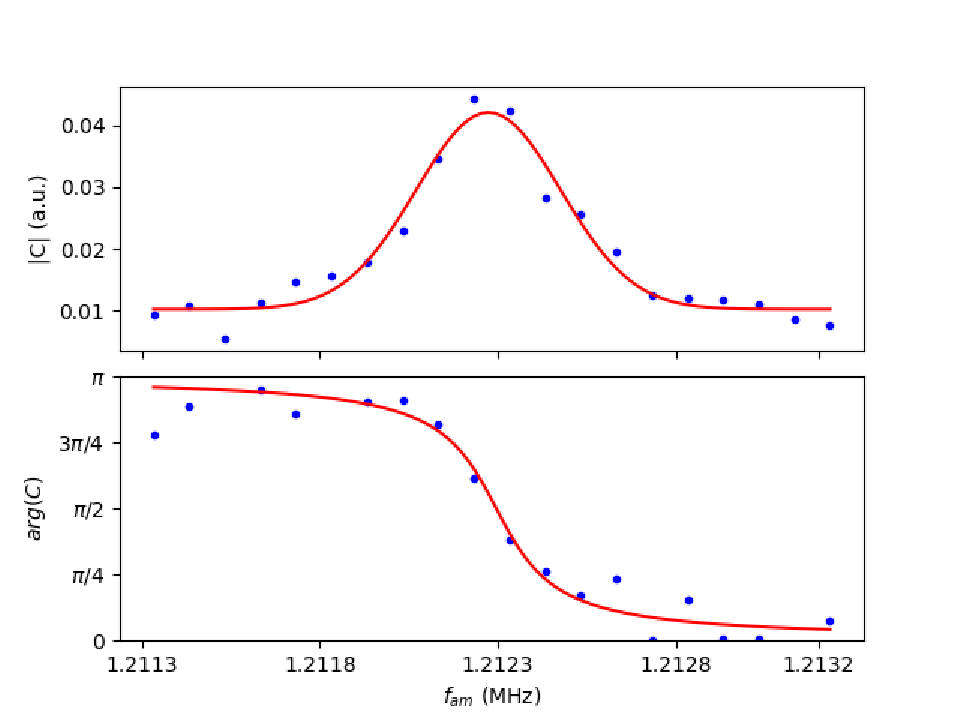
\includegraphics[width=0.4\linewidth]{fig_2_pe_x.pdf}}
    \caption{Parametric excitation approach for minimizing excess micromotion.}
    \label{fig:fig_2_pe}
\end{figure}

By scanning the modulation frequency across \(\omega_x\), which indicates the resonant frequency, it is obvious that there is a phase shift of \(\pi\). This phase shift may be aided further by the peak value of \(c_{-1}\) that occurs during a frequency scan. The sensitivity is influenced by two factors: (a) the modulation factor h, and (b) the degree to which the modulation frequency is detuned with respect to the secular frequency. Notice that there is a correction to the secular frequency that is related to the modulation, but that it is not represented here. The fundamental physics, however, remains the same.



\section{Coherent manipulation of ions}

The ${ }^{171} \mathrm{Yb}^{+}$ qubits are the primary research topic in our laboratory, the qubit itself is encoded in the ground state manifold's two hyperfine levels. In order to manipulate the qubit using a laser, one must make use of the Raman transition, which is facilitated by various auxiliary energy levels.

\subsection{Theory of laser-ion interaction}

In this part, I will focus on the interaction of a single ion with the laser. The application of this concept to the situation of several ions is quite simple, with the exception of the laborious indexing required for the normal mode ladder operators. The Halmitonian for the trapped ion that was irradiated by the laser is as follows:
\begin{equation}
    \hat{H} = \hat{H}_0 + \hat{V},
\end{equation}
where $\hat{H}_0$ refers to the non-interacting component and $\hat{V}$ refers to the interaction part. After being cooled by Doppler cooling, it is possible to safely view it as a harmonic oscillator, even if there is just a single ion trapped in the potential. And if we are just concerned with a two-level internal system and a z-axis exterior motion of the ion, then (we shall set $\hbar$ as 1 in the following)
\begin{equation}
    \hat{H}_0=\omega_0 /2 \hat{\sigma}_z + \nu \hat{a}^{\dagger} \hat{a},
\end{equation}
where $\omega_0$ operator for the annihilation of the z-axis motion. We now deduce the laser-ion interaction, denoted by the symbol $\hat{V}$; however, we only take into account the electric-field component of the laser and use a semi-classical point of view. This means that the laser field is not quantized,
\begin{equation}
    \mathbf{E}=\frac{\mathbf{E}_0}{2}\left(e^{i\left(\omega_L t-\mathbf{k} \cdot \mathbf{R}+\varphi_L\right)}+e^{-i\left(\omega_L t-\mathbf{k} \cdot \mathbf{R}+\varphi_L\right)}\right),
\end{equation}
where $\mathbf{R}$ represents the position vector of the ion, $\mathbf{E}_0$ represents the amplitude of the laser field, $\omega_L$ represents the frequency of the laser field, and $\varphi_L$ represents the phase of the laser field. In this context, we will use the example of dipole interaction. The location of the ion along the z axis may be expanded by the ladder operator,
\begin{equation}
    \hat{z}=\bar{z} + z_0 (\hat{a}^{\dagger}+\hat{a}),
\end{equation}
where $\bar{z}$ is the average position, $z_0$ is the motional extent, and $\hat{a}\, (\hat{a}^{\dagger})$ was just described above. The motional extent is the distance traveled by the ion along the z axis. The dipole interaction Hamiltonian might therefore be written as
\begin{equation}
    \hat{V}=-e\left(\mathbf{r}_{e g} \hat{\sigma}_{+}+\mathbf{r}_{e g} \hat{\sigma}_{-}\right) \cdot \frac{\mathbf{E}_0}{2}\left(e^{i\left(\omega_L t-\eta\left(\hat{a}^{\dagger}+\hat{a}\right)+\phi\right)}+\text { H.c. }\right),
\end{equation}
where $\mathbf{r}_{e g}=\langle e|\hat{\mathbf{r}}| g\rangle, \hat{\sigma}_{+}\left(\hat{\sigma}_{-}\right)$is $|e\rangle\langle g|(|g\rangle\langle e|), \eta=z_0 k \cos \theta$ is a parameter derived from the Lamb-Dicke equation that describes the relationship between the ion-motional extent and the laser wavelength. This parameter is often considerably less than $1$, and in our configuration, it is between $0.07-0.09$ away from a transverse mode.
\begin{equation}
    \phi = \varphi_L - k\cos{\theta} \bar{z}
\end{equation}
is just a re-defined laser phase factor. In all those formulas that we have derived before, the symbol $\theta$ refers to the angle that exists between the laser wave vector $\mathbf{k}$ and the ion-motional axis z. We put the whole Hamiltonian into the interaction picture of the uncoupled Hamiltonian, $\hat{H}_0$ with
\begin{equation}
    \hat{U}_0= e^{i \hat{H}_0 t},
\end{equation}
\begin{equation}
    \begin{aligned}
        \hat{H}_I & =\hat{U}_0 \hat{H} \hat{U}_0^{\dagger}-i \hat{U}_0 \frac{\partial \hat{U}_0^{\dagger}}{\partial t}                                                                                                                                                                               \\
                  & =-e\left(\mathbf{r}_{e g} \hat{\sigma}_{+} e^{i \omega_0 t}+\mathbf{r}_{e g} \hat{\sigma}_{-} e^{-i \omega_0 t}\right) \cdot \frac{\mathbf{E}_0}{2}\left(e^{i\left(\omega_L t-\eta\left(\hat{a}^{\dagger} e^{i v t}+\hat{a} e^{-i v t}\right)+\phi\right)}+\text { H.c. }\right)
    \end{aligned}
    .
\end{equation}

By using the rotating wave approximations (RWA), we are able to eliminate the high frequency components, which are on the order of $\omega_L+\omega_0$, and get the Hamiltonian that is associated with the interaction picture,
\begin{equation}
    \hat{H}_I=-e \mathbf{r}_{e g} \cdot \frac{\mathbf{E}_0}{2} \hat{\sigma}_{+} e^{-i(\delta t+\phi)} e^{i \eta\left(\hat{a}^{\dagger} e^{i v t}+\hat{a} e^{-i v t}\right)}+H.c.,
\end{equation}
where $\delta = \omega_L-\omega_0$ is the detuning. We decided to go with
\begin{equation}
    \Omega=-e \mathbf{r}_{e g} \cdot \mathbf{E}_0 e^{-i \phi},
\end{equation}
which is known as the Rabi frequency, then the $\hat{H}_I$ is
\begin{equation}\label{eq:1}
    \hat{H}_I=\frac{\Omega}{2} \hat{\sigma}_{+} e^{-i \delta t} e^{i \eta\left(\hat{a}^{\dagger} e^{i v t}+\hat{a} e^{-i v t}\right)}+\text { H.c. }.
\end{equation}

We make the observation that this Hamiltonian is generated from the dipole interaction, nevertheless, for any other sort of interactions, whether quadrupole or Raman interaction, the Hamiltonian of laser and ion is always of the same form. The only thing that is different is the concrete representation of the Rabi frequency, which is denoted by $\Omega$, however, we are not too concerned about it since it can be determined by experimentation. As the ytterbium hyperfine qubits are the primary research topic in our laboratory, I will provide an in-depth depiction of the Raman interaction in the next part.

Let us proceed by assuming the following form for the detuning $\delta$ of the laser frequency $\omega_L$ from the atomic frequency $\omega_0$,
\begin{equation}
    \delta=\omega_L-\omega_0=k\nu, \ k=0,\pm1,\pm2,\dots
\end{equation}

We apply BCH theorem \footnote{$e^{X} e^{Y}=e^{Z}$ where $Z=X+Y+\frac{1}{2}[X, Y]+\frac{1}{12}[X,[X, Y]]-\frac{1}{12}[Y,[X, Y]]+\cdots$} to equation \eqref{eq:1},
\begin{equation}
    \label{2}
    \hat{H}_I=\frac{\Omega}{2} \hat{\sigma}_+ e^{-\eta^2/2}\sum_{n,m=0}^{\infty} (i\eta)^{n+m}\frac{(a^\dagger)^n}{n!}\frac{a^m}{m!}e^{i\nu t (n-m-k)} + H.c.
\end{equation}

If the laser is tuned at the frequency $\omega_L$ such that $k=0$, the spectral line is called the carrier. For $k>0$ ($k<0$), the spectral line is termed the $k$th blue (red) sideband because the laser is blue (red) detuned from the atomic frequency $\omega_0$.

The spectral line is referred to as the carrier when the laser is adjusted to operate at the frequency $\omega_L$ in such a way that $k=0$. Since the laser is blue (or red) detuned from the atomic frequency $\omega_0$, the spectral line is referred to as the $k$th blue (or red) sideband when $k>0$ (or $k<0$), respectively.

As a result, the Hamiltonian of the kth order, denoted by the symbol $\hat{H}_I^k$, may be written as follows,

For $k>0$
\begin{equation}
    \hat{H}_I^k=\sum_{m=0}^{\infty}\left(\frac{\Omega_{m, m+k}}{2}|e\rangle\langle g|\otimes| m+k\rangle\langle m|+\text { H.c. }\right),
\end{equation}

For $k<0$
\begin{equation}
    \hat{H}_I^k=\sum_{m=0}^{\infty}\left(\frac{\Omega_{m, m+|k|}}{2}|e\rangle\langle g|\otimes| m\rangle\langle m+|k||+H . c .\right),
\end{equation}

\begin{equation}
    \Omega_{m,m+k}=\Omega_{m+k,m}=\Omega e^{-\eta^2/2}(i\eta)^{k}L_m^{k}(\eta^2)\sqrt{\frac{m!}{(m+k)!}}
\end{equation}
is the Rabi frequency between the two states, $|g\rangle|m\rangle(|g\rangle|m+k\rangle)$ and $|e\rangle|m+k\rangle(|e\rangle|m\rangle)$.
\begin{equation}
    \Omega_{m, m+k}=\left|\Omega_{m, m+k}\right| e^{i \frac{k \pi}{2}-i \phi}.
\end{equation}

The $\hat{U}_{k}=\exp(-i\hat{H}_I^k t)$ notation denotes the temporal evolution operator. In order to discover the rule, we may broaden it and do the calculation $(\hat{H}_I^k)^2$, $(\hat{H}_I^k)^3$.

We are primarily interested in the interactions on the carrier ($k = 0$) and the first red (blue) sideband ($k=-1(+1)$) in terms of quantum coherent manipulations of a single ion. This is because these interactions are the fundamental components for the constructions of a wide class of quantum manipulations, such as sideband cooling and the spin-dependent force.

For $k=0$
\begin{equation}
    \begin{aligned}
        \hat{U}_c & =\sum_{m=0}^{\infty} \cos \left(\frac{\left|\Omega_{m, m}\right| t}{2}\right)(|g\rangle\langle g|\otimes| m\rangle\langle m|+| e\rangle\langle e|\otimes| m\rangle\langle m|) \\
                  & -i \sum_{m=0}^{\infty} \sin \left(\frac{\left|\Omega_{m, m}\right| t}{2}\right)\left(|e\rangle\langle g|\otimes| m\rangle\langle m| e^{-i \phi}+\text { H.c. }\right)
    \end{aligned}
    .
\end{equation}

For $k=-1\, (+1)$
\begin{equation}
    \begin{aligned}
        \hat{U}_{r(b)} & =\sum_{m=0}^{\infty} \cos \left(\frac{\left|\Omega_{m, m+1}\right| t}{2}\right)(|g(e)\rangle\langle g(e)|\otimes| m+1\rangle\langle m+1|+| e(g)\rangle\langle e(g)|\otimes| m\rangle\langle m|)            \\
                       & -i \sum_{m=0}^{\infty} \sin \left(\frac{\left|\Omega_{m, m+1}\right| t}{2}\right)\left(|e\rangle\langle g|\otimes| m(m+1)\rangle\langle m+1(m)| e^{i\left(\frac{\pi}{2}-\phi\right)}+\text { H.c. }\right)
        \\
                       & +|g(e)\rangle\langle g(e)|\otimes| 0\rangle\langle 0|
    \end{aligned}
    .
\end{equation}

Even when the average phonon number of the motional state is rather large, the preceding forms may still be applied to the dynamics of the ions even while operating outside of the Lamb-Dicke regime. The majority of the time, especially after ground-state cooling of the ion motion, we only expand the Hamiltonian \eqref{eq:1} to the first order of the Lamb-Dicke parameter $\eta$ in the Lamb-Dicke regime. After doing so, the Hamiltonian \eqref{eq:1} can be approximated to
\begin{equation}
    \label{10}
    \hat{H}_I=\frac{\Omega}{2} (\hat{\sigma}_+ e^{-i\delta t}+H.c.) +\frac{i\eta\Omega}{2}\left(\hat{\sigma}_+ (\hat{a}^\dagger e^{i(\nu-\delta) t} + \hat{a}e^{-i(\nu+\delta) t})+H.c.\right).
\end{equation}

This is especially true after ground-state cooling of the ion motion. Setting $\delta$ close to $0$, $-\nu$ and $\nu$ accordingly and disregarding the rather rapid rotating terms allows us to quickly get the carrier, the first red sideband, and the first blue sideband from this equation.

\subsection{Raman coherent control}

Now consider how the Raman laser beams would react if the Raman laser beam came into contact with a single ion. This laser is called a pump laser. Its frequency is $\omega_p$ and Rabi frequency is $\Omega_p$. The other laser is called a Stokes laser. Its frequency is $\omega_s$ and Rabi frequency is $\Omega_s$. As we can see from Fig.~\ref{fig:Raman}, there are two laser beams coupling the spin-down state ($\left|\downarrow\right\rangle$) and the auxiliary state ($\left|1\right\rangle$). The laser-ion Hamiltonian under intraction picture is an extension of the equation that additionally considers the cross coupling terms (i.e. the pump (Stokes) beam also couples $|\uparrow(\downarrow)\rangle$ and $|1\rangle$), as well as the intraction picture.
\begin{equation}
    \begin{aligned}
        \label{Raman interaction H}
        \hat{H}_{R} & =\left(\frac{\Omega_p^{1\uparrow}}{2}\hat{\sigma}_{1\uparrow}e^{-i(\Delta+\omega_0)t}+\frac{\Omega_p^{1\downarrow}}{2}\hat{\sigma}_{1\downarrow}e^{-i\Delta t}\right)e^{i\eta_p(a^\dag e^{i\nu t}+ae^{-i\nu t})} \\&+\left(\frac{\Omega_s^{1\uparrow}}{2}\hat{\sigma}_{1\uparrow}e^{-i(\Delta-\delta)t}+\frac{\Omega_s^{1\downarrow}}{2}\hat{\sigma}_{1\downarrow}e^{-i(\Delta-\delta-\omega_0) t}\right)e^{i\eta_s(a^\dag e^{i\nu t}+ae^{-i\nu t})}+H.c.,
    \end{aligned}
\end{equation}
where $\Omega_x^{i, j}=-\frac{e \mathbf{r}_{i, j} \cdot \mathbf{E}_x}{\hbar} e^{-i \phi_x}(i, j=\downarrow, \uparrow, 1$ and $x=p, s)$ means the Rabi frequency coupling $|i\rangle$ and $|j\rangle$ via laser $x$ and $\hat{\sigma}_{i, j}=|i\rangle\langle j|$. $\Delta$, $\delta$ and $\omega_0$ is explained in the caption of Fig.~\ref{fig:Raman}.

\begin{figure}
    \centering
    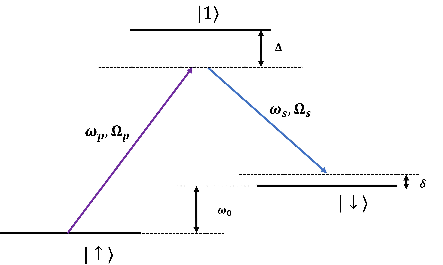
\includegraphics[width=0.7\linewidth]{fig_2_Raman.pdf}
    \caption{Level scheme of Raman transition.}
    \label{fig:Raman}
\end{figure}

Changing to a new reference frame via $\hat{U}=e^{i \delta t|\uparrow\rangle\langle\uparrow|+i \Delta t| 1\rangle\langle 1|}$ allows us to get the Hamiltonian, which is as follows,
\begin{equation}
    \begin{aligned}
        \widetilde{H} & =-\delta|\uparrow\rangle\langle\uparrow|-\Delta| 1\rangle\langle 1|+\left[\left(\frac{\Omega_p^{1 \downarrow}}{2} \sigma_{1 \downarrow}+\frac{\Omega_p^{1 \uparrow}}{2} \sigma_{1 \uparrow} e^{-i\left(\omega_0+\delta\right) t}\right) e^{i \eta_p\left(a^{\dagger} e^{i v t}+a e^{-i v t}\right)}\right. \\
                      & \left.+\left(\frac{\Omega_s^{1 \uparrow}}{2} \sigma_{1 \uparrow}+\frac{\Omega_s^{I \downarrow}}{2} \sigma_{1 \downarrow} e^{i\left(\omega_0+\delta\right) t}\right) e^{i \eta_s\left(a^{\dagger} e^{i v t}+a e^{-i v t}\right)}+H . c .\right] .
    \end{aligned}
\end{equation}

For $\delta\ll\omega_0$, and $\Omega_s^{1\downarrow},\Omega_p^{1\uparrow} \ll \omega_0+\delta$, it might be possible to omit the cross-coupling phrases. The Hamiltonian equation would therefore be,
\begin{equation}
    \begin{aligned}
        \breve{H} & =-\delta|\uparrow\rangle\langle\uparrow|-\Delta| 1\rangle\langle 1|                                                                                                                                                                                                            \\
                  & +\left[\frac{\Omega_p^{1 \downarrow}}{2} \hat{\sigma}_{1 \downarrow} e^{i \eta_p\left(a^{\dagger} e^{i v t}+a e^{-i v t}\right)}+\frac{\Omega_s^{1 \uparrow}}{2} \hat{\sigma}_{1 \uparrow} e^{i \eta_s\left(a^{\dagger} e^{i v t}+a e^{-i v t}\right)}+\text { H.c. }\right] .
    \end{aligned}
\end{equation}

If we set the internal state as
\begin{equation}
    |\psi(t)\rangle=c_{\downarrow}(t)|\downarrow\rangle+c_{\uparrow}(t)|\uparrow\rangle+c_1(t)|1\rangle,
\end{equation}
then the evolution equations of $c_{\downarrow},c_{\uparrow},c_1$ are
\begin{equation}
    \begin{aligned}
        i \dot{c}_{\downarrow} & =\frac{\left(\Omega_p^{1 \downarrow}\right)^*}{2} e^{-i \eta_p\left(a^{\dagger} e^{i v t}+a e^{-i v t}\right)} c_1                                                                                                                 \\
        i \dot{c}_{\uparrow}   & =-\delta c_{\uparrow}+\frac{\left(\Omega_s^{1 \dagger}\right)^*}{2} e^{-i \eta_s\left(a^{\dagger} e^{i v t}+a e^{-i v t}\right)} c_1                                                                                               \\
        i \dot{c}_1            & =\frac{\Omega_p^{1 \downarrow}}{2} e^{i \eta_p\left(a^{\dagger} e^{i v t}+a e^{-i v t}\right)} c_{\downarrow}+\frac{\Omega_s^{1 \dagger}}{2} e^{i \eta_s\left(a^{\dagger} e^{i v t}+a e^{-i v t}\right)} c_{\uparrow}-\Delta c_1 .
    \end{aligned}
\end{equation}

If that $\Delta$ is far larger than $\Omega^{1\downarrow}_p$ and $\Omega^{1\uparrow}_s$, the population probability of $|1\rangle$ will be very low due to the far detuning. Hence, we will be able to adiabatically remove this irrelevant state by setting $\dot{c}_1$ to zero and obtaining  $c_1=\frac{\Omega^{1\downarrow}_P c_{\downarrow}+\Omega^{1\uparrow}_s c_{\uparrow}}{2\Delta}$. The effective equation for the development of a system with two levels is as follows,
\begin{equation}
    \begin{aligned}
        i \dot{c}_{\downarrow} & =\Lambda_{\downarrow} c_{\downarrow}+\frac{\Omega_R^*}{2} e^{-i \eta\left(a^{\dagger} e^{i v t}+a e^{-i v t}\right)} c_{\uparrow}                 \\
        i \dot{c}_{\uparrow}   & =\frac{\Omega_R}{2} e^{i \eta\left(a^{\dagger} e^{i v t}+a e^{-i v t}\right)} c_{\downarrow}+\left(\Lambda_{\uparrow}-\delta\right) c_{\uparrow},
    \end{aligned}
\end{equation}

$\Lambda_{\downarrow(\uparrow)}=\frac{\left|\Omega_{p(s)}^{1, \downarrow(\uparrow)}\right|^2}{4 \Delta}$ is the second-order AC Stark shift of the state, $\eta=\eta_p-\eta_s$ is the Lamb-Dicke parameter of the differential wave vector $\Delta \mathbf{k}=\mathbf{k}_p-\mathbf{k}_s$. The effective Rabi frequency used to couple the two qubit states is denoted by $|\downarrow(\uparrow)\rangle$ and $\Omega_R=\frac{\Omega^{1\downarrow}_p \times (\Omega^{1\uparrow}_s)^*}{2\Delta}$. Now, with the help of the aforementioned evolution equations, we can easily get the effective Hamiltonian of the qubit,
\begin{equation}
    \hat{H}_{\mathrm{eff}}=\frac{\Delta_{s s}}{2} \hat{\sigma}_z+\frac{\Lambda_{\uparrow}+\Lambda_{\downarrow}}{2} \hat{I}-\delta \hat{\sigma}_{+} \hat{\sigma}_{-}+\left(\frac{\Omega_R}{2} e^{i \eta\left(a^{\dagger} e^{i v t}+a e^{-i v t}\right)} \hat{\sigma}_{+}+H . c .\right),
\end{equation}
where $\Delta_{ss}=\Lambda_{\uparrow}-\Lambda_{\downarrow}$ is the differential AC Stark shift of the two qubit levels. By removing an insignificant component from $\hat{I}$ and transferring into the reference frame in terms of $\hat{U}_0=e^{-i\delta\hat{\sigma}_+\hat{\sigma}_-+i\Delta_{ss}\sigma_z/2}$, we get the effective Hamiltonian that is identical to Eq.~\eqref{eq:1},
\begin{equation}
    \hat{H}_{\mathrm{eff}}=\frac{\Omega_R}{2} e^{-i \mu t} e^{i \eta\left(a^{\dagger} e^{i v t}+a e^{-i v t}\right)} \hat{\sigma}_{+}+H . c .,
\end{equation}
where $\mu=\delta-\Delta_{ss}$ is a redefinition of the two-photon detuning. On the basis of this Hamiltonian, it is feasible to do all of the manipulations, such as switching between the carrier and the red and blue sidebands.
